\documentclass[a4paper]{article}

\usepackage[T1]{fontenc}
\usepackage[utf8]{inputenc}
\usepackage[swedish]{babel}
\usepackage{csquotes}
\usepackage{hyperref}
\usepackage{url}
\usepackage[pdftex]{graphicx}
\usepackage[flushleft]{threeparttable}
\usepackage{booktabs}
\usepackage{amsmath}

\title{DSCS - EDAA40/EDAA75}

\begin{document}

\maketitle

\section{DNF}

\begin{figure}[ht]
	\centering
	\resizebox{\textwidth}{!}{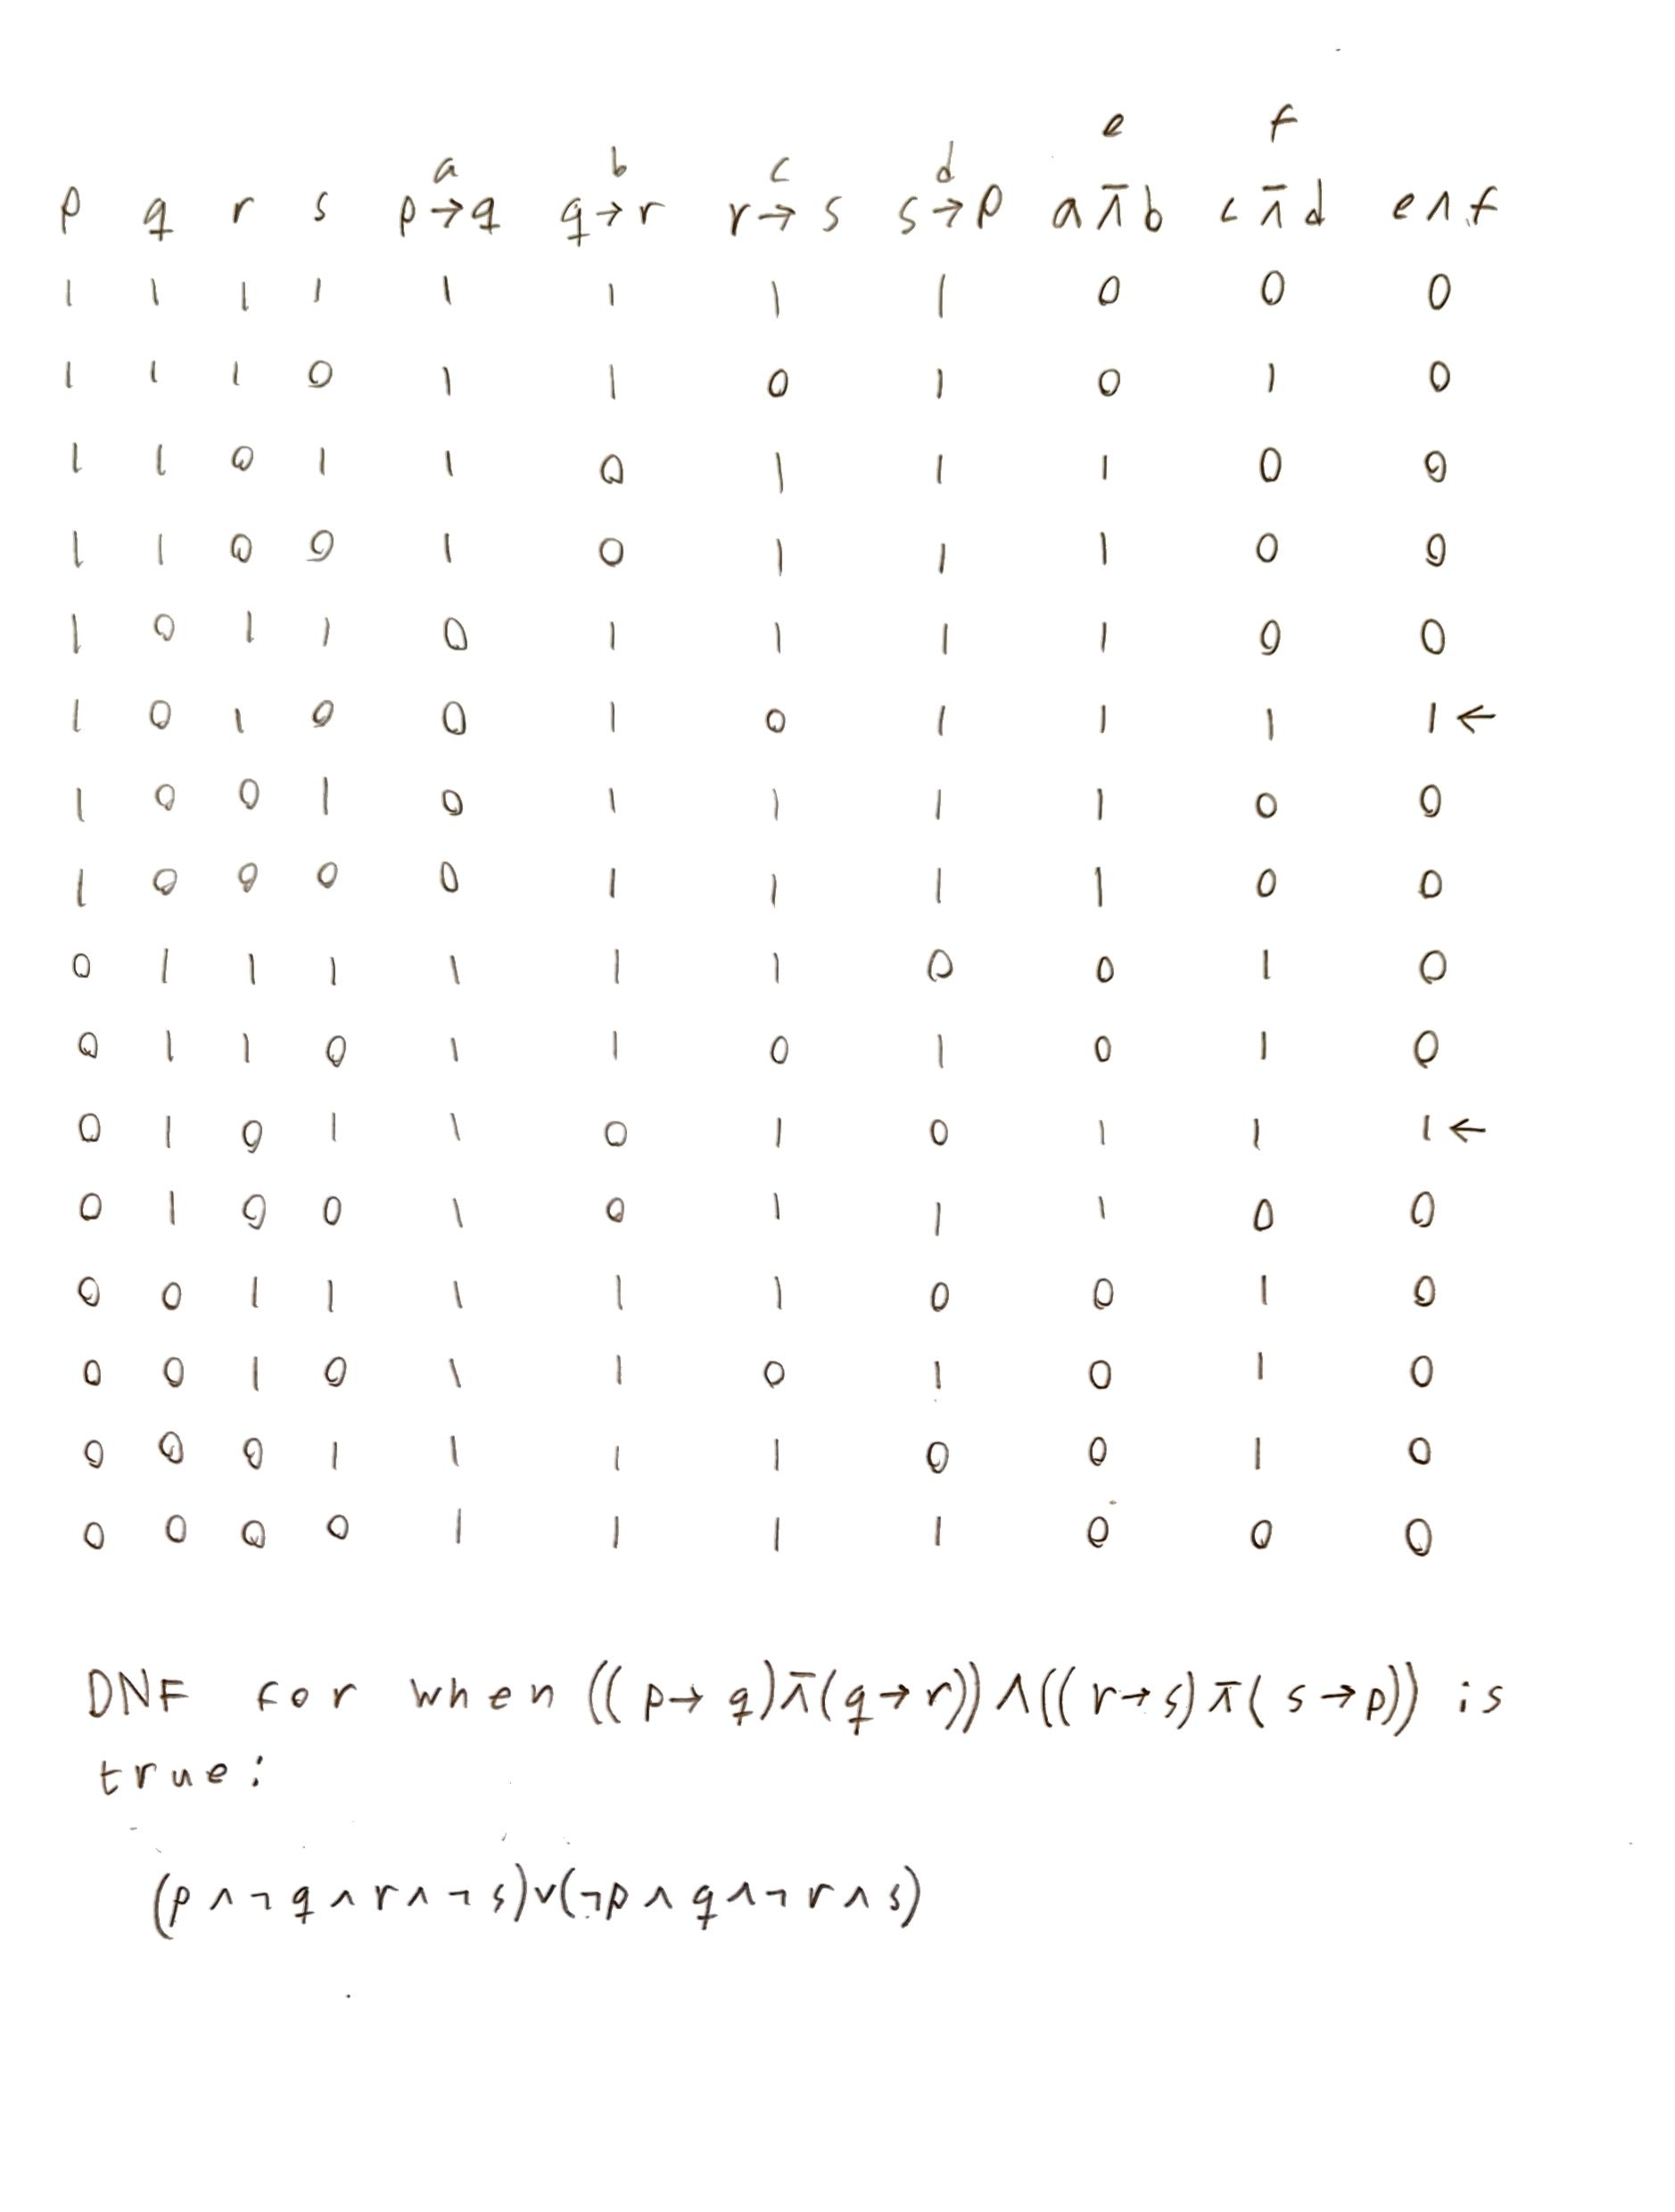
\includegraphics{2018_1/solution-5.1.jpeg}}
	\caption{För att lösa DNF uppgifter kan man skapa ett truth table med alla literaler som förekommer i uttrycket.
  Sedan bygger man stegvis upp hela uttrycket med fler kolumner.
	}\label{fig:2018-5-1}
\end{figure}

\end{document}
